Neutrino physics is at the core of current high energy research. One of the profound discoveries made in recent years was the observation of neutrino flavour oscillations by the Super-Kamiokande experiment, which was the first confiramtion that physics existed beyond the standard model of particle physics. In brief, neutrinos described by the standard model would be massless particles, but since the flavours are made up of superpositions of mass states, the oscillation of
the flavour states implies that the relative mass states are different, and therefore non-zero \cite{nuInt}.

    Future, long-baseline,  neutrino experiments such as the Deep Underground Neutrino Experiment (DUNE) and Hyper-Kamiokande (Hyper-K) are hoping to investigate some of the most fundamental questions we are still asking: Why does the universe constist of matter, and not anti-matter? What is the neutrino mass heirarchy?

    Neutrino research is an extremely active field. Optimising the current and future detectors to maximise the accuracy of all interaction anaylses is a crucial step towards obtaining concrete answers to these questions. 

    A brief introduction to the topics covered in this report is as follows, more detail on each will be given in later sections. 

\subsection{Neutrino interactions}

Due to the elusive nature of the neutrino, directly observing one in a detector isn't possible. It is therefore necessary to infer their existence from particles produced when they interact. Since this process relies upon the reconstruction capability of the experiment, purpose-built detectors will attempt to maximise the efficiency of this.

Another property of the neutrino which poses a significant difficulty within detectors is their interaction probability, or cross-section. A typical neutrino cross-section is on the order of $ 10^{-44} $ cm$^{2}$ which translates to $\sim$1 interaction every 10 light years in steel, for neutrinos with only a few MeV energy \cite{nuOsc}. This fact introduces the need for the interacting neutrinos to have high energies in these dedicated experiments, if we are to sufficiently reduce their mean free path.

More detail on this topic will be discussed in section~\ref{sec:NIP}.

\subsection{GENIE}

    GENIE is the world leading neutrino interaction generator. Generators are a crucial machinery in all high energy physics analyses as they use theoretical models to produce predictions of how and where neutrino interactions will occur in specific detector geometries. With this information, comparisons between experimental data and theoretical predictions can be drawn, the models can be updated and potential new physics can be explored.

    Generators such as GENIE bridge the gap between theory and experiment, whilst also providing opportunities to prepare simulations and perform sensitivity studies for the next generation of neutrino experiments.

    GENIE's role in current and future neutrino experiments will be discussed further in section~\ref{sec:GF}.

\subsection{Cross-sections}
   
    In order to correctly model neutrino events within a specific detector geometry and material, certain parameters have to be known. In particular, the probability of an interaction taking place - its cross-section - is required for each possible interaction the neutrino could undergo. Cross-section measurements are therefore a necessity for the generators, and consequently the future detector studies mentioned earlier. 
    
    Our current knowledge of charged current neutrino cross sections is given in \cite{xsecCurr}. 

    %CC cross-sections
    \begin{figure}[h!]
        \center
        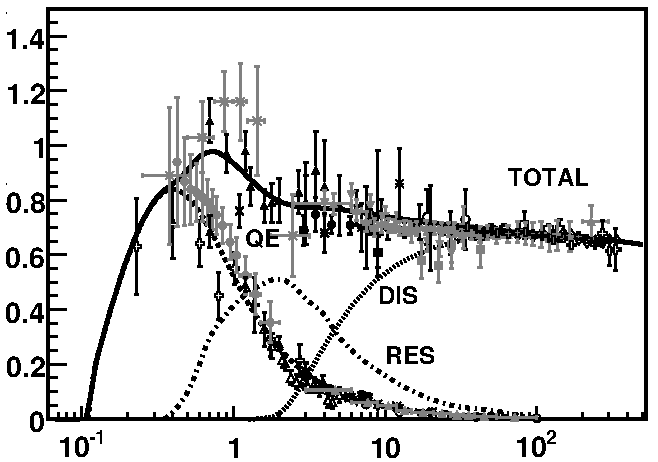
\includegraphics[width=.8\textwidth]{images/current_cross_sec_knowledge.pdf}
        \caption{ Cross-section knowledge to date}
        \label{fig:xsecCurr}
    \end{figure}

    
    % Plan
    \begin{itemize}

        \item Why?
        
        \begin{itemize}

            \item Simulation
            \item GENIE

        \end{itemize}
        
        \item Historical
        \item Current knowledge
        \item Needs for future
        
        \begin{itemize}

            \item LArTPCs
            \item Statistics

        \end{itemize}

    \end{itemize}

\subsection{GENIE-Professor global fits}


\clearpage
